%%%%%%%%%%%%%%%%%%%% author.tex %%%%%%%%%%%%%%%%%%%%%%%%%%%%%%%%%%%
%
% sample root file for your "contribution" to a contributed volume
%
% Use this file as a template for your own input.
%
%%%%%%%%%%%%%%%% Springer %%%%%%%%%%%%%%%%%%%%%%%%%%%%%%%%%%


% RECOMMENDED %%%%%%%%%%%%%%%%%%%%%%%%%%%%%%%%%%%%%%%%%%%%%%%%%%%
\documentclass[graybox]{svmult}

% choose options for [] as required from the list
% in the Reference Guide

\usepackage{mathptmx}       % selects Times Roman as basic font
\usepackage{helvet}         % selects Helvetica as sans-serif font
\usepackage{courier}        % selects Courier as typewriter font
\usepackage{type1cm}        % activate if the above 3 fonts are
                            % not available on your system
%
\usepackage{makeidx}         % allows index generation
\usepackage{graphicx}        % standard LaTeX graphics tool
                             % when including figure files
\usepackage{multicol}        % used for the two-column index
\usepackage[bottom]{footmisc}% places footnotes at page bottom

% see the list of further useful packages
% in the Reference Guide

\begin{document}


% media synchronization
\begin{table}
\centering
\caption{Common challenges for media synchronization on the Web.}
\label{tab:challenges}
\setlength{\tabcolsep}{10pt}
\begin{tabular}{cc}
\hline\noalign{\smallskip}
Synchronization challenges & Use-cases \\
\noalign{\smallskip}\svhline\noalign{\smallskip}
across media sources & multi-angle video, ad-insertion \\
across media types & video, WebAudio, animated map \\
across iframes & video, timed ad-banner \\
across tabs, browsers, devices & split content, interaction \\
across platforms & Web, native, broadcast \\
across people and groups & collaboration, social \\
across Internet & global media experiences \\
\noalign{\smallskip}\hline\noalign{\smallskip}
\end{tabular}
\end{table} 


\begin{figure}[h]
%\sidecaption
\centering
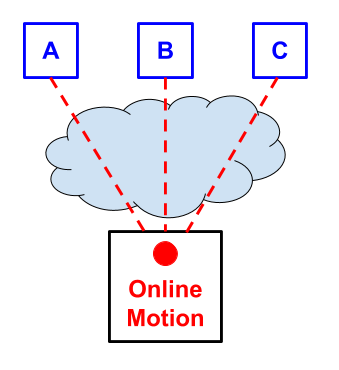
\includegraphics[scale=.4]{fig/motion-model.png}
\caption{Media components on three different devices (A,B,C), all connected to an online motion
(red circle). Media control requests (e.g. pause/resume) target the online motion and are transmitted across the Internet (light blue cloud). The corresponding state change is
communicated back to all connected media components. Each media component
adjusts its behaviour independently.}
\label{fig:model}
\end{figure}

\begin{figure}[h]
%\sidecaption
\centering
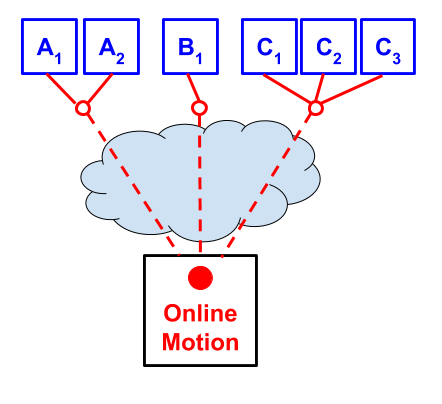
\includegraphics[scale=.4]{fig/motion-model-2.png}
\caption{Timing objects (red unfilled circles) mediate access to online motion. Timing objects may be shared by independent media components within the same browing context.}
\label{fig:model-2}
\end{figure}

\begin{figure}[h]
%\sidecaption
\centering
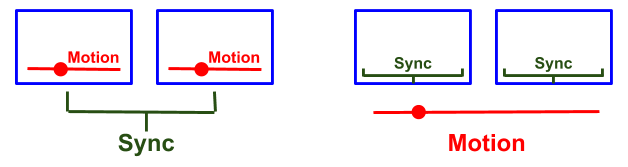
\includegraphics[scale=.4]{fig/internal-external.png}
\caption{
  Blue rectangles represent media components, red symbols represent motion, and green symbols represent the process of media synchronization. To the left: internal timing and external media synchronization. To the right: external timing and internal media synchronization.
}
\label{fig:internalexternal}
\end{figure}


\begin{figure}[h]
%\sidecaption
\centering
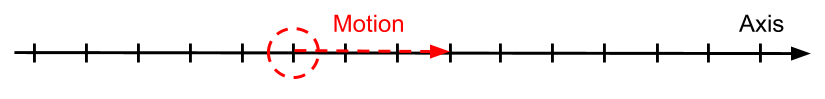
\includegraphics[scale=.4]{fig/motion-axis.png}
\caption{Motion: point moving along an axis. The current position
is marked with a red circle (dashed), and forward velocity of 3 units per second is
indicated by the red arrow (dashed).}
\label{fig:motion}
\end{figure}

\begin{figure}[h]
%\sidecaption
\centering
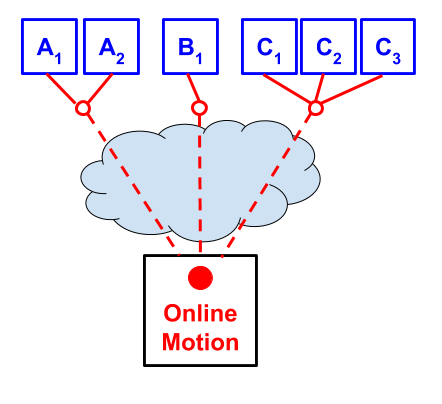
\includegraphics[scale=.3]{fig/motion-model-2.png}
\caption{(Fig.~\ref{fig:model-2} repeated for convenience.) Timing objects (red unfilled circles) mediate access to online motion. Timing objects may be shared by independent media components within the same browsing context.}
\label{fig:model-repeat}
\end{figure}

\begin{figure}[h]
%\sidecaption
\centering
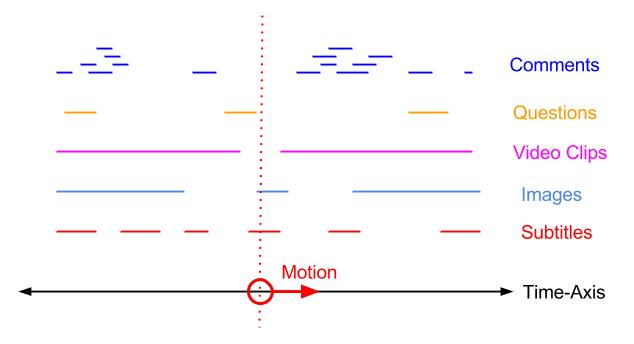
\includegraphics[scale=.4]{fig/sequencer.jpg}
\caption{Five data sources of timed data, with items tied to intervals on the timeline. Motion along the same timeline defines which items are active (vertical dotted line), and precisely when items will be activated or deactivated.}
\label{fig:sequencer}
\end{figure}

\begin{figure}[h]
%\sidecaption
\centering
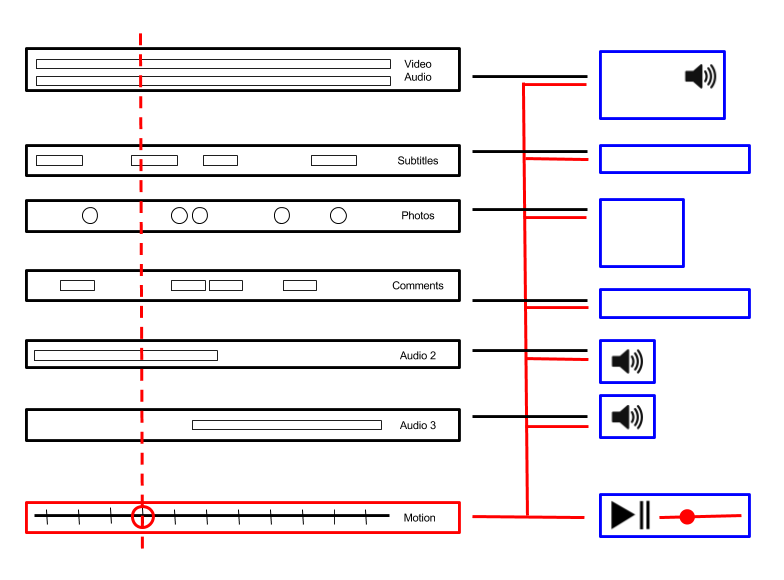
\includegraphics[scale=.4]{fig/motion-media.png}
\caption{A single media experience made from multiple media components (blue), possibly distributed across multiple devices. Each media component is connected to motion (red) and a source of timed data (black). There are different types of timed data: an AV container, a subtitle track, photos, comments and two extra audio tracks. The motion defines the timeline for the presentation, and timed data is mapped to this timeline by each media component. Since all the media components are connected to the same motion, they will operate in precise synchrony. One particular media component (bottom media element) provides interactive controls for the presentation, and connects only with motion.}
\label{fig:motion-media}
\end{figure}

\begin{figure}[h]
%\sidecaption
\centering
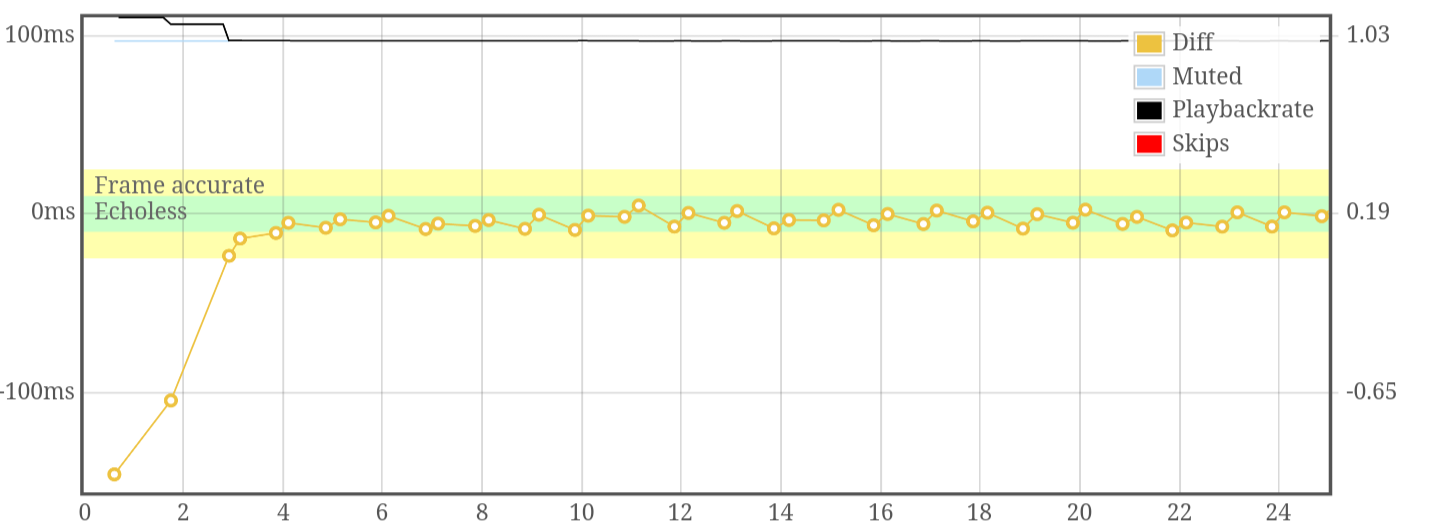
\includegraphics[scale=.23]{fig/android-video.png}
\caption{The figure illustrates an experiment with video (mp4) synchronization on
Android using Chrome browser. The plot shows currentTime compared to the ideal
playback position defined by motion. The X-axis denotes the timeline of the experiment (seconds).
The left Y-axis denotes difference \emph{Diff} (milliseconds) between currentTime and motion.
The green band (echoless) is +-10 millisecond and the yellow (frame accurate is) +-25 millisecond. 
This is achived using variable playbackRate. No skips were performed in this experiment. 
The right Y-axis denotes the value of playbackrate (seconds per second). The media element was muted until playbackrate stabilized.}
\label{fig:videosync}
\end{figure}


\end{document}
